\chapter{An Overview on Proteins}
\label{chp:proteins}

\section{Basics of Molecular Biology}
\subsection{Cells}
Life is made of cells, the fundamental working units of every living system. They are composed of :
\begin{itemize}
	\item 70\% of water;
	\item 23\% of macromolecules, such as:
	\begin{itemize}
		\item proteins;
		\item polysaccharides.
	\end{itemize}
	
	\item 7\% of small molecules, such as:
	\begin{itemize}
		\item lipids;
		\item amino acids;
		\item nucleotides.
	\end{itemize}
\end{itemize}
Cells are the smallest structural unit of an organism capable of independent functioning.Each cell follows the same common cycle of birth, replication, protein synthesis and death. 

Cells have common features in their structure, in the next page I will show a figure, representing the main components of a cell.

\pagebreak

\begin{figure}[h!]
	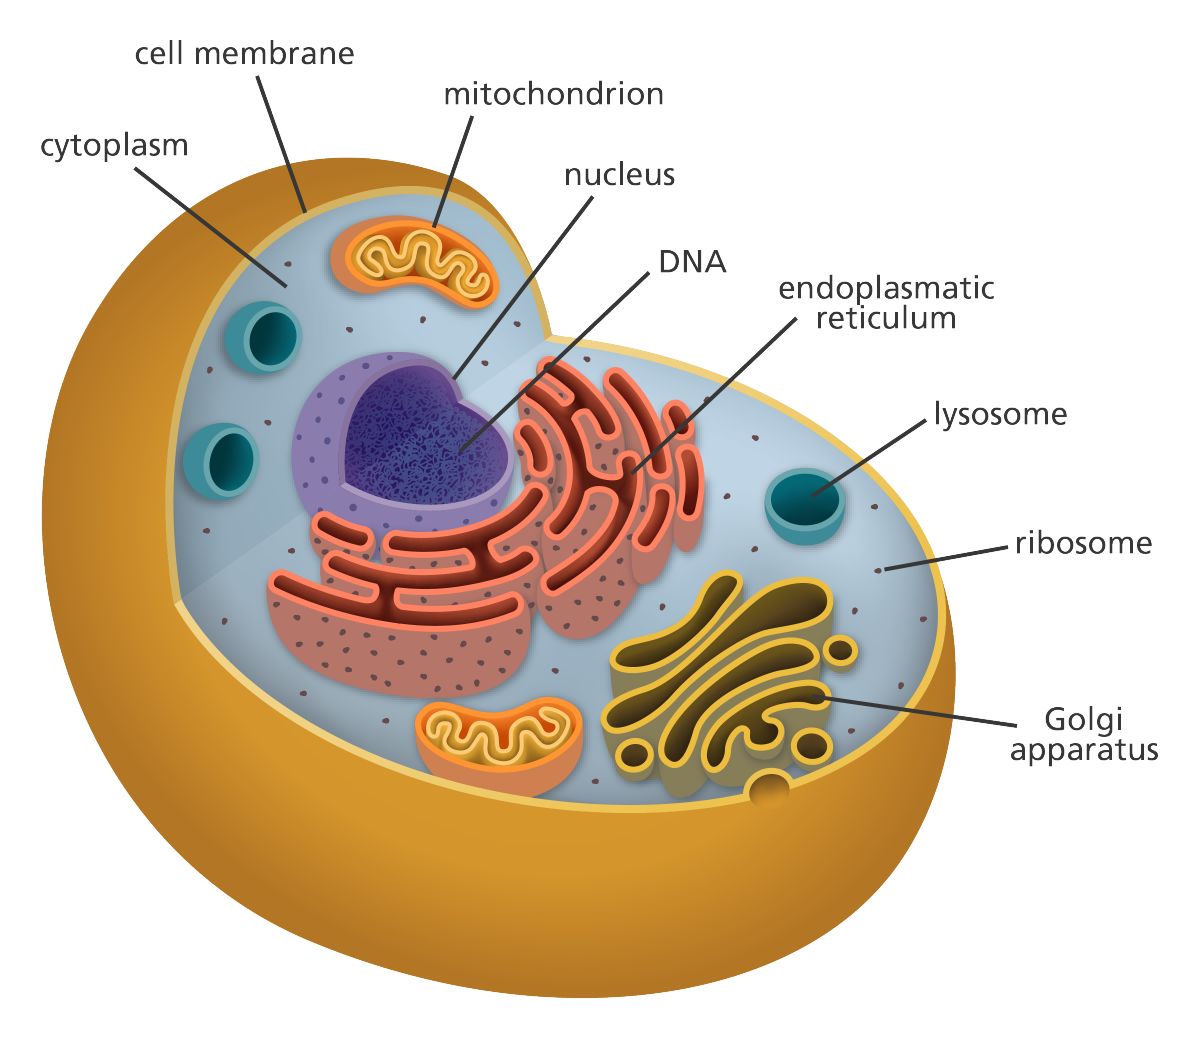
\includegraphics[scale=.25]{res/proteins_overview/cell_structure.png}
	\centering
	\caption{Cell structure}
	\label{fig:cell-structure}
\end{figure}

Let's analyse the main components among the ones we can see from the figure \ref{fig:cell-structure}:
\begin{itemize}
	\item \textbf{Nucleus}: it's the main component of the cell which contains the DNA, the genetic information of the individual. Around the nucleus there is the nucleus membrane, not annotated in the figure, that separates the nucleus from the cytoplasm;
	\item \textbf{Golgi apparatus}: or Golgi vesicles. Its purpose is to help processing and packaging the molecules, especially proteins that will be exported from the cell;
	\item  \textbf{Mitochondria}: they are one of the most important cellular organelles, since they generate most of the chemical energy, the ATP, to power the cell's biochemical reactions. They generate the ATP through aerobic respiration;
	\item \textbf{Cytoplasm}: a gelatinous liquid that fills the inside of the cell, it's made of water, salts and various enzymes. It has many purposes, such as giving the cell a specific shape, protecting the cell organelles and assisting the cell's metabolic processes;
	\item \textbf{Cell membrane}: also called plasma membrane, is a semipermeable membrane that separates the interior of the cell from the outside environment. This membrane regulates the transport of molecules entering and exiting the cell, thanks to its semipermeability.
\end{itemize}
There are other elements we didn't describe in a cell, such as the endoplasmic reticulum and some cell organelles such as peroxisome, lysosome, ribosome, secretory vesicles and others.
\subsection{DNA}
The nucleus of the cell contains the DNA, which is the genetic information of the individual. It might slightly change between cells, especially among different types of cells, such as muscle cells and brain cells, since their functionalities are different.
\subsubsection{Chromosomes}
The genome is an organism's complete set of DNA, the human genome contains about 3 billion DNA base pairs and 24 distinct chromosomes. 

\begin{figure}[h]
	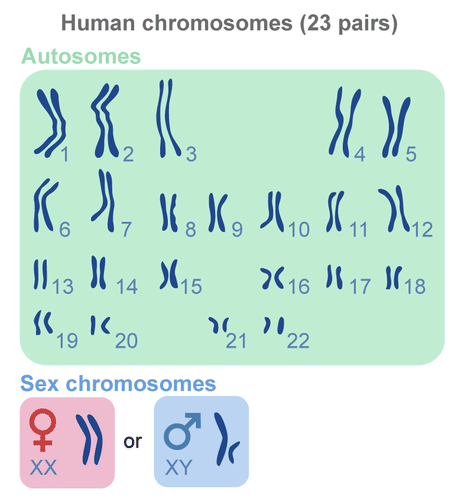
\includegraphics[scale=0.8]{res/proteins_overview/chromosomes.png}
	\caption{Chromosomes set in human genome}
	\label{fig:chromosomes}
\end{figure}

In figure \ref{fig:chromosomes} we can see the set of 24 chromosomes in the human genome. A cell normally contains 23 chromosomes, the 22 common ones, the autosomes, plus one of the sex chromosomes, "XX" in females and "XY" in males.
\subsubsection{Genes}
Each chromosome contains many genes, the basic functional units of heredity. Genes are specific sequences of DNA that encode instructions on how to make proteins.


\begin{wrapfigure}{l}{0.5\textwidth} %this figure will be at the right
	\centering
	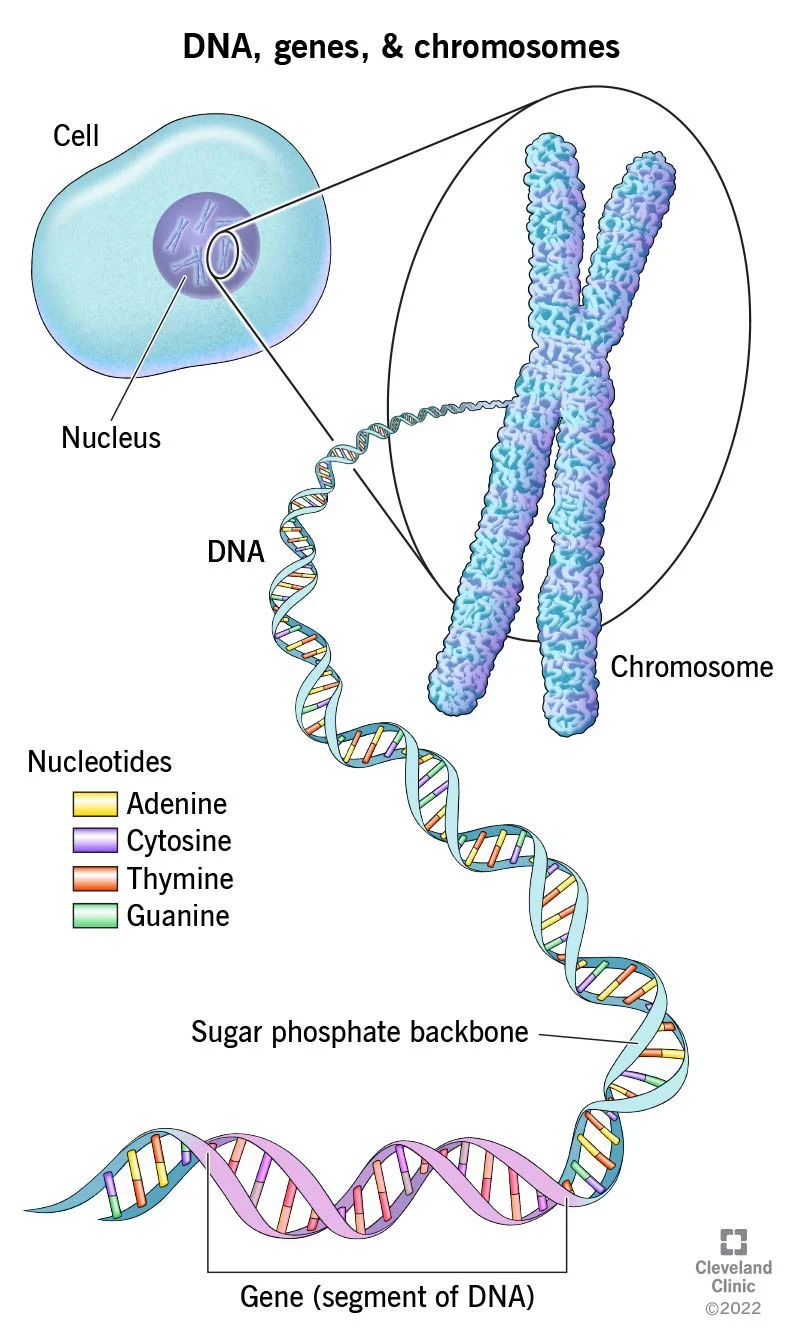
\includegraphics[width=0.5\textwidth]{res/proteins_overview/genes.png}
\end{wrapfigure}

From the figure on the left we can see how genes, along with the DNA, fold into chromosomes, which will contain a really high density of DNA. Finally the chromosomes will be stored inside the nucleus of the cell.

Genes determine the principal hereditary stuff in the human being, from the height, to growth, muscular mass and appetite. Some of these elements are defined by a group of genes, others from just a singular gene. Mutations of some genes can modify the characteristics of a human and they can make alterations as harmless as a different eye color or they can result in more serious outcomes, like diseases. These mutations can also provide beneficial effects, such as immunity or protection for some diseases, for example a specific gene mutation is known for its protection against malaria.

Genes are vastly studied, especially their function in the DNA: some genes are highly related to diseases, such as:
\begin{itemize}
	\item Huntington disease;
	\item Down syndrome;
	\item Cystic fibrosis;
	\item Albinism;
	\item various types of cancer.
\end{itemize}

\subsubsection{DNA structure}

\begin{figure}[h!]
	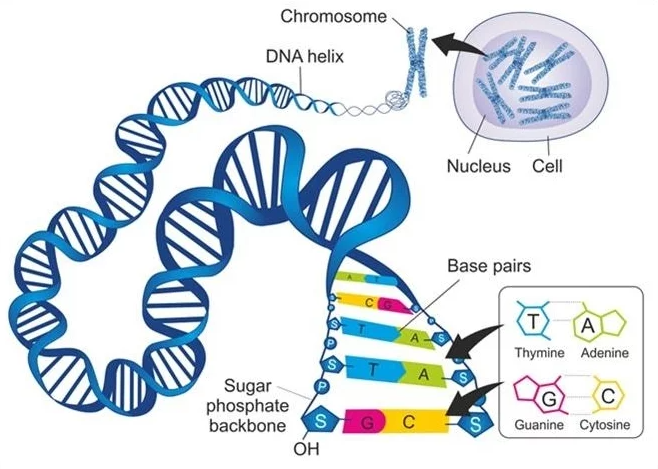
\includegraphics[scale=.6]{res/proteins_overview/dna_basepairs.png}
	\centering
	\caption{DNA structure}
	\label{fig:dna-structure}
\end{figure}

The figure \ref{fig:dna-structure} represents the DNA structure, a double helix macromolecule composed of nucleotides. A nucleotide is a molecule composed of:
\begin{itemize}
	\item \textbf{Sugar phosphate backbone}: a molecule of sugar combined with a group phosphate;
	\item \textbf{Nitrogenous base}: there are four possible bases in DNA:
	\begin{itemize}
		\item Adenine;
		\item Thymine;
		\item Guanine;
		\item Cytosine.
	\end{itemize}
\end{itemize}
The nucleotides pair up with the nucleotides of the opposite helix, via the nitrogenous base: the only possible pairs are Adenine-Thymine and Guanine-Cytosine.

\pagebreak

The DNA can replicate itself or can be used to produce proteins, which are particular molecules that participate in most of the essential processes of the human body:
\begin{itemize}
	\item building and repairing body structures;
	\item digesting nutrients;
	\item hormones: some hormones are proteins or protein-derived. Hormones are chemical messengers that flow through blood to coordinate different body's functions;
	\item executing various metabolic functions, or assisting the execution.
\end{itemize}
We will now see more in detail this process from DNA to proteins, called protein synthesis.

\subsection{Central Dogma of Biology}
\label{sec:central-dogma}
\begin{figure}[h!]
	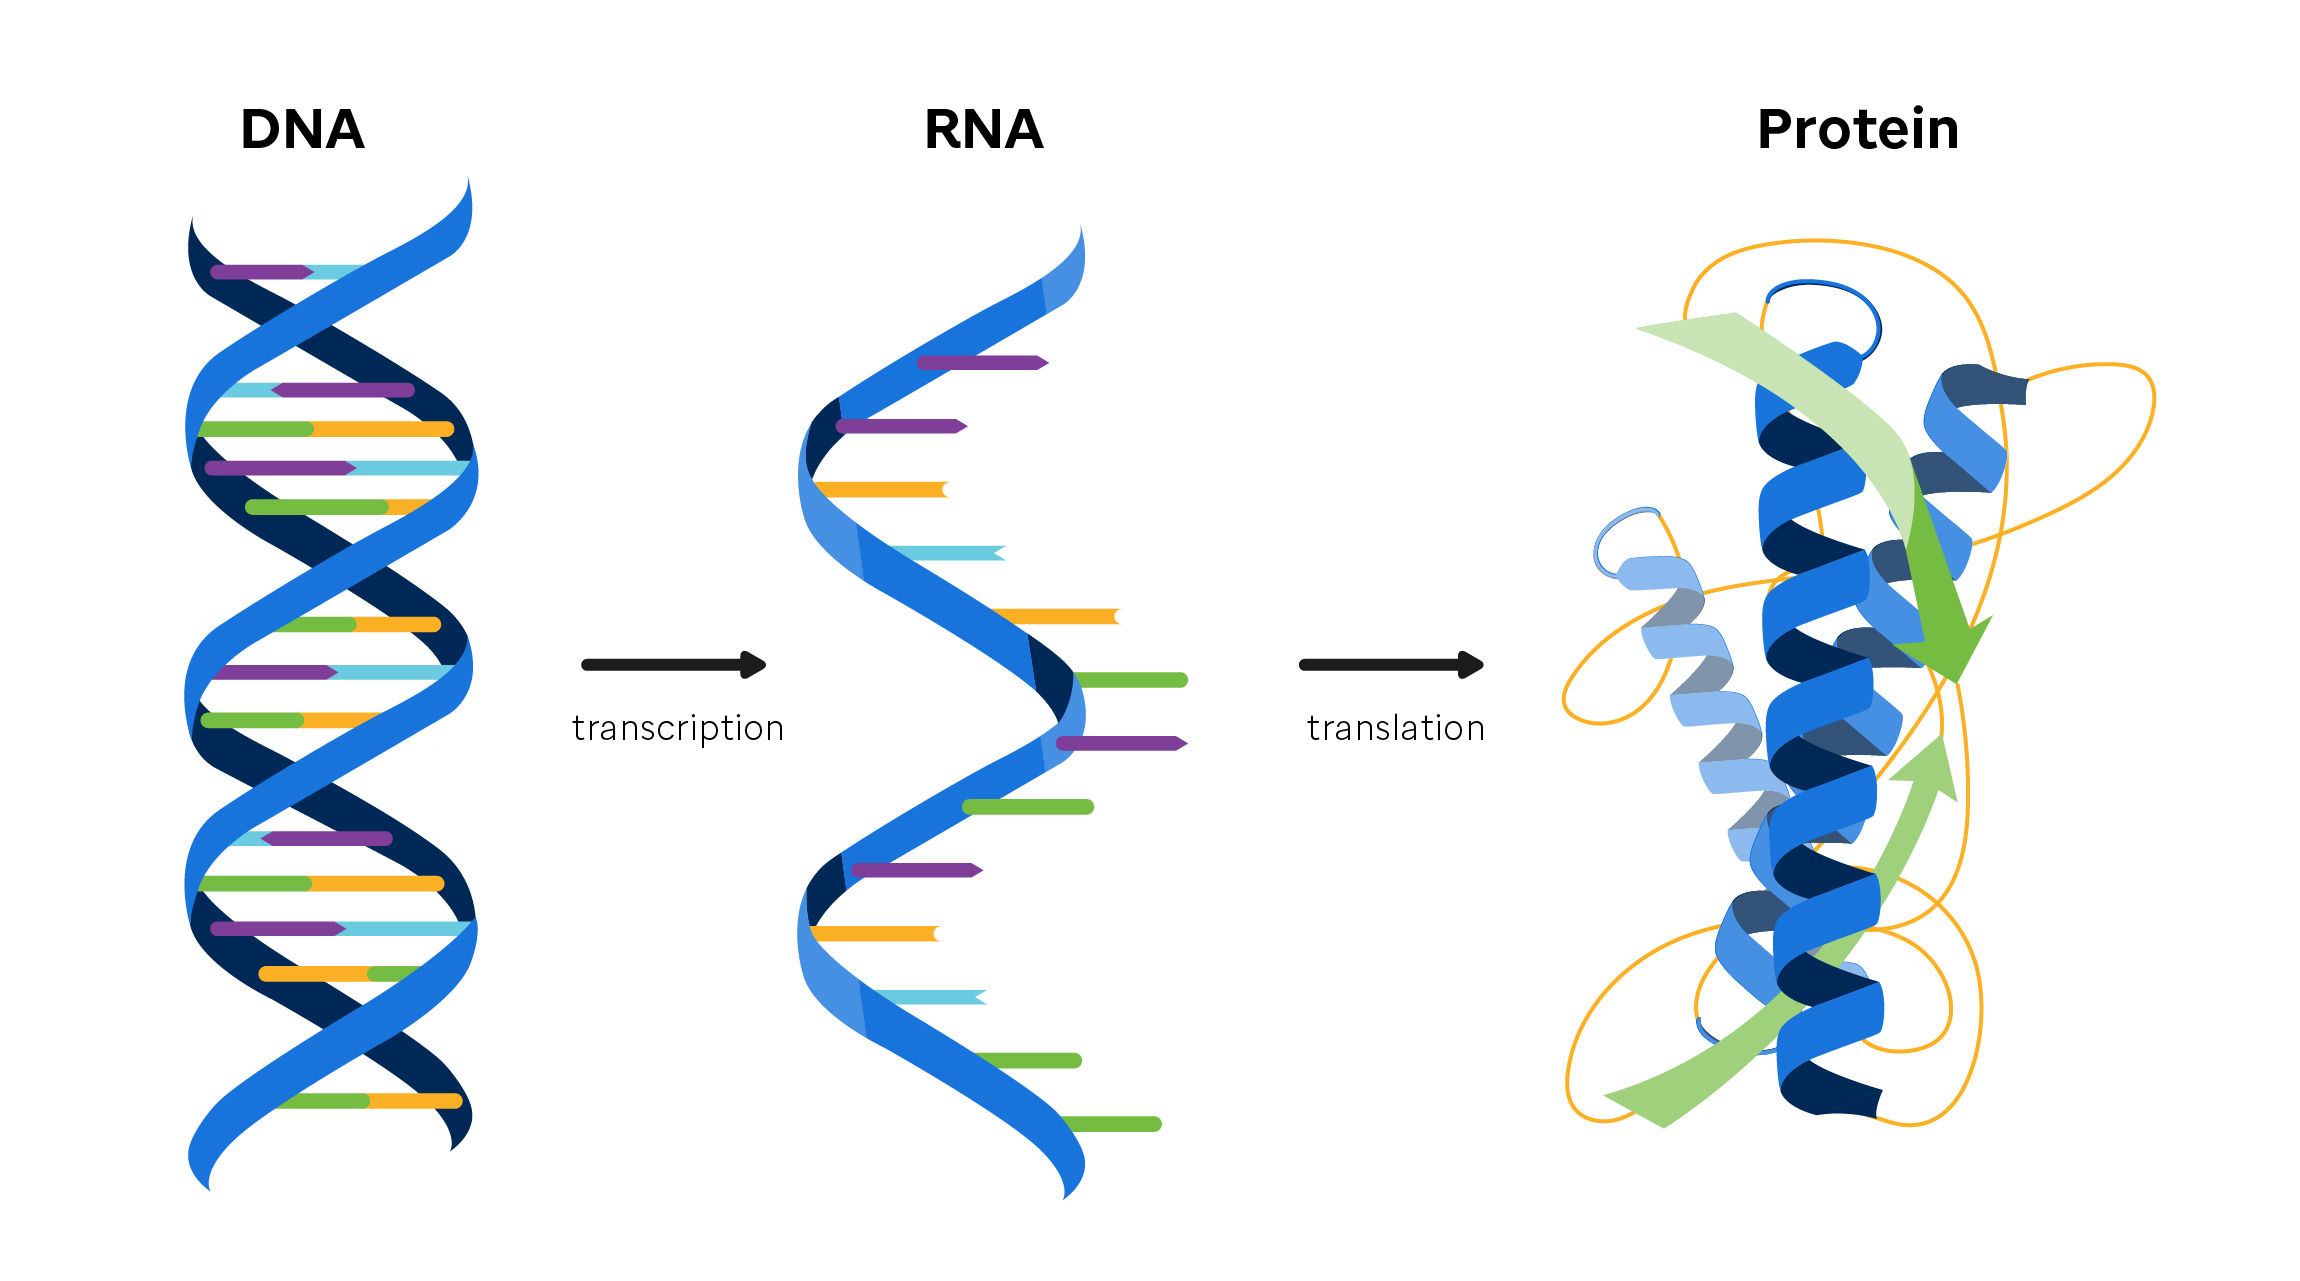
\includegraphics[scale=.27]{res/proteins_overview/central_dogma.png}
	\centering
	\caption{Central Dogma of Biology}
	\label{fig:central-dogma}
\end{figure}

The figure \ref{fig:central-dogma} represents the Central Dogma of Biology, which explains the flow of genetic information within a biological system: from DNA to RNA to protein.

\pagebreak

\subsubsection{Transcription}
Transcription is the process of copying a segment of DNA into RNA. An enzyme called RNA polymerase produces an RNA strand, by passing through a DNA strand. The resulting RNA is the copy of the coding strand of the "input" DNA , while the strand used as template to create this copy is called template strand.

\begin{figure}[h!]
	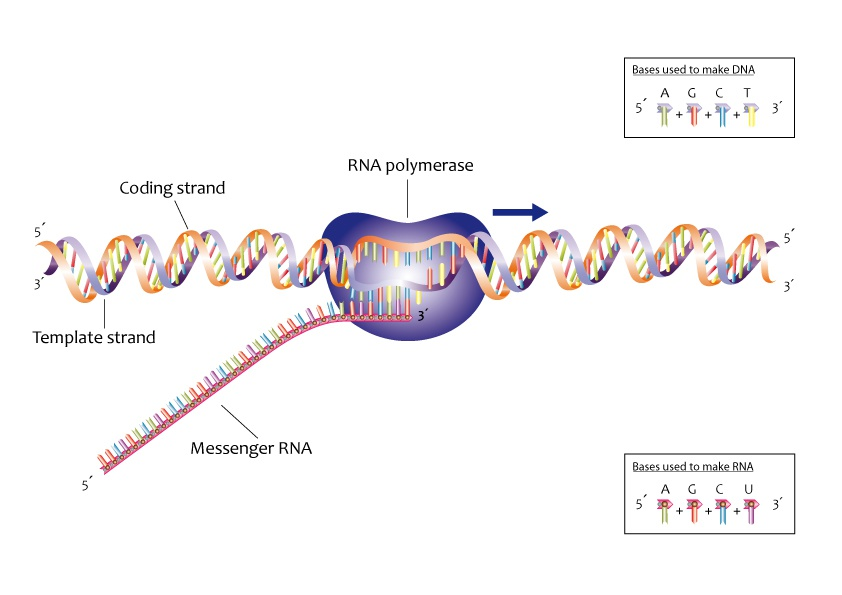
\includegraphics[scale=.6]{res/proteins_overview/rna_polymerase.jpeg}
	\centering
	\caption{Central Dogma of Biology}
	\label{fig:transcription}
\end{figure}

In the figure above, we can see how RNA polymerase creates the RNA. We can note that in the figure the RNA is called messenger RNA, also known as \textbf{mRNA}.

There are other two types of RNA, tRNA and rRNA. Let's see the differences:
\begin{itemize}
	\item \textbf{mRNA}: messenger RNA, contains the genetic information from the DNA. mRNA specifies ;
	\item \textbf{tRNA}: transfer RNA, transfer the correct amino acid to the ribosome. It acts as a bridge between the mRNA and the ribosome;
	\item \textbf{rRNA}: ribosomal RNA, combined with ribosomal proteins creates the ribosome.
\end{itemize}
\subsubsection{Translation}
Translation is the process by which the genetic information from the DNA is converted into a functional protein. It's also known as protein synthesis.

The ribosome reads the following three nucleotides of the mRNA, this triplet is the \textbf{codon}, then the ribosome brings in the correct tRNA. The correct tRNA is the tRNA, whose triplet, the \textbf{anticodon}, matches the actual triplet of the mRNA.
Once we have a matched tRNA, the tRNA transfers the amino acid to the growing protein chain of the ribosome.

\begin{figure}[h!]
	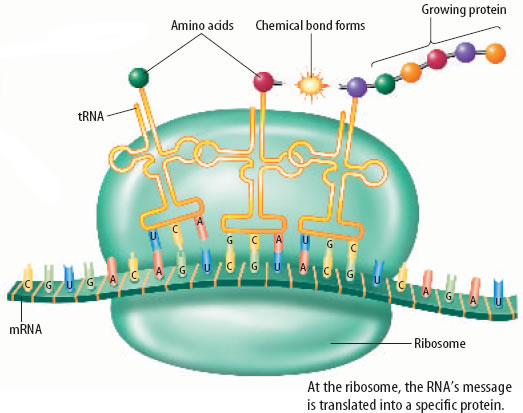
\includegraphics[scale=.6]{res/proteins_overview/protein_synth.jpeg}
	\centering
	\caption{Protein Synthesization}
	\label{fig:protein-synth}
\end{figure}

In figure \ref{fig:protein-synth} we can see how the ribosome, along with tRNAs, identifies the correct amino acid and transfers it into the growing protein, through a chemical bond.

\begin{figure}[h!]
	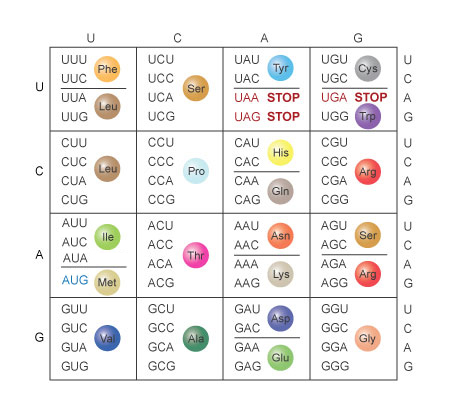
\includegraphics[scale=1.4]{res/proteins_overview/genetic_code.png}
	\centering
	\caption{Genetic code}
	\label{fig:genetic-code}
\end{figure}

In the figure \ref{fig:genetic-code} above, we can observe the Genetic Code: the set of triplets of nucleotides, codons and the corresponding amino acid.

We can observe 4 particular combinations of nucleotides that correspond to signal of start and stop the protein synthesization:
\begin{itemize}
	\item The codon \textbf{AUG} identifies the \textbf{START} signal for the protein translation;
	\item The codons \textbf{UAA, UAG, UGA} identify the \textbf{STOP} signal, which ends the translation process producing the final protein.
\end{itemize}
\vspace{5em}
\subsection{Proteins}
Proteins are large, complex molecules made up of amino acids, smaller subunits also referred to as residues. The residues are the building blocks of a macromolecule, so in this case the residues are the incorporated amino acids.
Proteins are linear chains of different combinations of 20 different amino acids. 

\subsubsection{Proteins' Functions}
\begin{itemize}
	\item Make up the cellular structure;
	\item Form body's major components, such as skin and hairs;
	\item Form hormones to communicate with other cells;
	\item Form enzymes to regulate gene activity.
\end{itemize}

The functions of proteins depend both on the amino acids' order and types and on the three-dimensional structure the protein folds into.

\subsubsection{Protein Folding}
Proteins tend to fold into lowest energy three-dimensional conformation. They already begin to fold already when the amino acid chain is being formed during translation.

Different amino acids have different chemical properties and by interacting with each other the protein starts to fold adopting its functional structure.

The structure of the protein is really important for the protein's function:
\begin{itemize}
	\item Determines which amino acids are exposed outside the protein;
	\item Determines which substrates the protein can react with.
\end{itemize}

Substrates are molecules or compounds that participate in a chemical reaction, they are starting materials or reactants which are acted upon by enzymes or catalysts.
\vspace{6em}
\pagebreak

\begin{figure}[h!]
	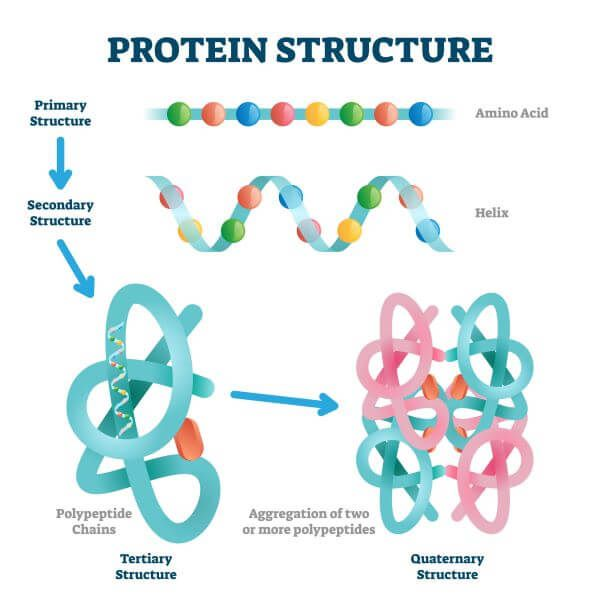
\includegraphics[scale=0.75]{res/proteins_overview/protein_structure.png}
	\centering
	\caption{Structure of proteins}
	\label{fig:protein-structure}
\end{figure}

From figure \ref{fig:protein-structure} we can see the four types of structures in a protein:

\begin{itemize}
	\item \textbf{Primary structure}: simply the sequence of amino acids;
	\item \textbf{Secondary structure}: local structural patterns formed by residues;
	\item \textbf{Tertiary structure}: the global structure of the peptide chain;
	\item \textbf{Quaternary structure}: the global structure and aggregation of the various peptide chains in the protein. 
\end{itemize}

\vspace{2em}

The main two types of secondary structures are :

\begin{itemize}
	\item \textbf{Alpha-helix}: proteins bury most of their hydrophobic residues in the interior core, forming a spiral structure resembling an helical spring;
	\item \textbf{Beta-sheets}: segments of the protein are stretched out and aligned in a sheet-like arrangement.
\end{itemize}
\vspace{6em}
\pagebreak
\subsubsection{Amino Acids}
Lastly, let's talk about the amino acids.
Amino acids are monomers\footnote{A monomer in molecular biology is a molecule that can bond with other monomers to create a macromolecule. } of proteins, each amino acid has a specific chemical behavior.
All amino acids in the human genetic code have a carboxyl group (-COOH) and an amino group (-NHH) bound to the central carbon atom. 

\vspace{2em}

\begin{figure}[h!]
	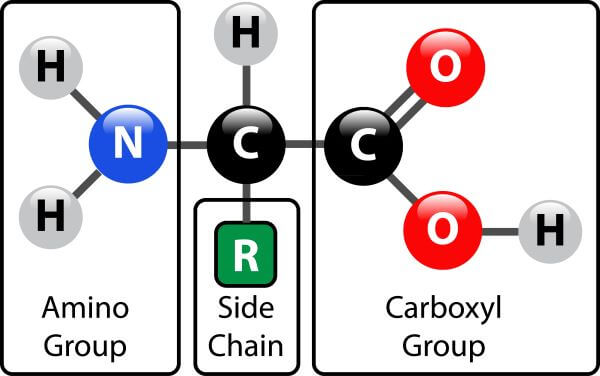
\includegraphics[scale=0.6]{res/proteins_overview/amino_structure.png}
	\centering
	\caption{Structure of amino acids}
\end{figure}

In the figure above, we can observe the general structure of amino acids in the human genetic code.

The carboxyl group and the amino group are the same for each one of the 20 amino acids, they differ for the side chain. Side chains differ in these 3 features :
\begin{itemize}
	\item three-dimensional structure;
	\item electric charge;
	\item hydrophobicity.
\end{itemize}

Amino acids are mainly classified by hydrophobicity :
\begin{itemize}
	\item hydrophobic amino acids repel water, they are also called non-polar amino acids. 
	\item hydrophilic amino acids are attracted to water, they are also called polar amino acids.
\end{itemize}
\pagebreak
Other classifications take into account the structure, functionality or electrical charge of the amino acid. The latter can be either uncharged, positively charged or negatively charged.
Some other classifications are based on the particularity of the side chains, such as Sulfur-Containing. Sulfur-Containing amino acids, as the name suggests, contain sulfur. 

\begin{table}[h!]
\begin{tabular}{ |c|c|c|c| }
	\hline
	 & & & \\
	\textbf{Full Name} & \textbf{Abbreviation} & \textbf{Abbreviation} & \textbf{Polarity} \\
	 & \textbf{(3 Letters)} & \textbf{(1 Letter)} & \\
	\hline
 Glycine & Gly & G & \\  
 Alanine & Ala & A & \\ 
 Valine & Val & V & \\
 Leucine & Leu & L & \\
 Isoleucine & Ile & I & Non-Polar \\
 Methionine & Met & M & \\
 Phenylalanine & Phe & F & \\
 Tryptophan & Trp & W & \\
 Proline & Pro & P & \\
 	\hline
 Serine & Ser & S & \\
 Threonine & Thr & T & \\
 Cysteine & Cys & C & \\
 Tyrosine & Tyr & Y & \\
 Asparagine & Asn & N & \\
 Glutamine & Gln & Q & Polar \\
 Aspartic Acid & Asp & D & \\
 Glutamic Acid & Glu & E & \\
 Lysine & Lys & K & \\
 Arginine & Arg & R & \\
 Histidine & His & H & \\
	\hline

\end{tabular}
\caption{List of Amino Acids}
\label{table:amino-acids}
\end{table}

\vspace{2em}

In the table \ref{table:amino-acids}, we can see the list of the 20 amino acids in the Genetic Code with :
\begin{itemize}
	\item Polarity;
	\item Three letters abbreviation;
	\item One letter abbreviation.
\end{itemize}

To check which triplet of nucleotides corresponds to each amino acid in the Genetic Code, we can go back to figure \ref{fig:genetic-code}.

\vspace{10em}

\subsection{Tandem Repeat Proteins}
Tandem repeat proteins are the product of minimal folds from the repetition of simpler units. Their buried residues are more conserved, with a large surface and a high sequence variability.

\begin{figure}[h!]
	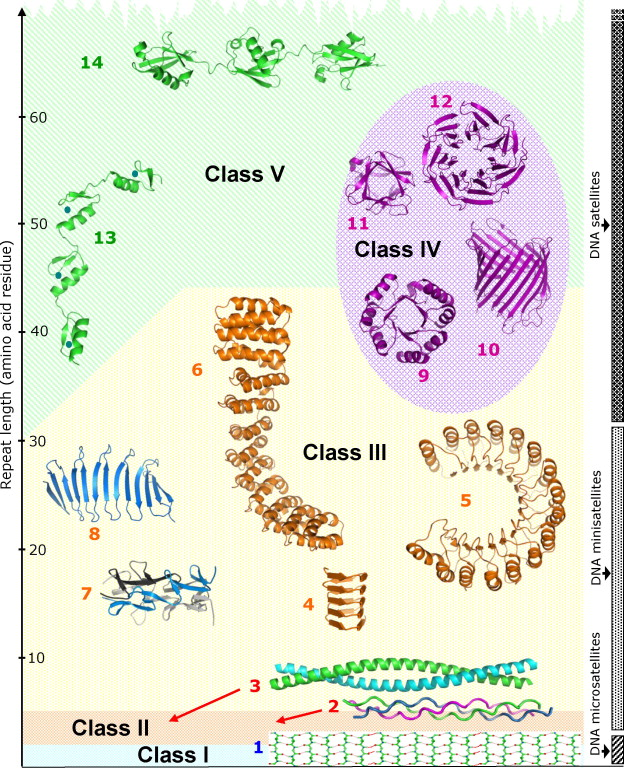
\includegraphics[scale=0.6]{res/proteins_overview/tandem.jpg}
	\centering
	\caption{Tandem Repeat Proteins}
	\label{fig:tandem}
\end{figure}

From the figure \ref{fig:tandem} we can see what tandem repeat proteins look like. We can also observe how they are divided into classes; tandem repeat proteins are classified according to periodicity in 5 classes:
\begin{itemize}
	\item Class I: Aggregates;
	\item Class II: Collagen and Coiled-coils;
	\item Class III: Solenoids;
	\item Class IV: Toroids;
	\item Class V: Beads on a string.
\end{itemize}

\subsection{Intrinsically Disordered Proteins}
A polypeptide chain can be classified as different types of proteins, such as:
\begin{itemize}
	\item Membrane proteins;
	\item Globular proteins;
	\item Tandem repeat proteins;
	\item Intrinsically disordered proteins.
\end{itemize}
We already saw Tandem Repeat Proteins, now we will explore Intrinsically Disordered Proteins.

\begin{figure}[h!]
	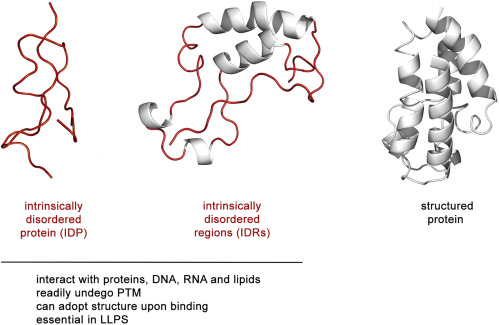
\includegraphics[scale=0.8]{res/proteins_overview/disordered.png}
	\centering
	\caption{Intrinsically Disordered Proteins}
	\label{fig:tandem}
\end{figure}
In disordered proteins the cost of folding is higher and so the protein has a lesser degree of freedom in folding.

It has complex surfaces which means high specificity with low versatility. For specificity we mean that when 2 proteins fit together, we need 2 highly specific protein structures to fit together, since their shape is so complex, an average protein can't be a proper fit.

Low versatility is the opposite: since the shape is quite complex, it doesn't fit together with most proteins, hence it's not versatile.

Due to their complex structures, disordered proteins are less prone to environmental stress: they can preserve their function in unstable conditions, such as high temperature.

In cell regulation around 25\% of proteins are disordered, those are involved in highly dynamic and complex processes that require proteins with high specificity.

IDPs (Intrinsically Disordered Proteins) are really interesting to study, because they are implicated in several pathologies and due to their different functions they are involved in:
\begin{itemize}
	\item Regulatory functions;
	\item Central role in the assembly of macromolecular machines, such as ribosomes;
	\item Transport of molecules through nuclear pore;
	\item Binding: IDPs can participate in one-to-many and many-to-many interactions, where one IDP region binds to multiple molecules, potentially gaining very different structures in the bound state.
\end{itemize}
 They are also implicated in several pathological conditions, like cancer, cardiovascular diseases, and neurodegenerative diseases. 

Some of the first classes of IDPs were notable due to their pathological roles in neurodegenerative diseases.

\vspace{20em}

\pagebreak

\section{Computational Biology: Computer Science Applied to Biology}
The growing amount of data in the field of Molecular Biology brought the scientists to exploit Computer Science. Computers can process data way faster than human beings, and especially in this field, where we have so much information on DNA, genes and proteins, it's really useful to compute and process these pieces of informations faster and possibly with less errors.

This new field takes the name of Bioinformatics, the union of Biology, Computer Science and Statistics. Statistics is needed because most of the information isn't 100\% reliable, hence statistics methods are used.
The main fields of bioinformatics are:
\begin{itemize}
    \item \textbf{Structural data analysis}: its purpose is to predict the three-dimensional structures of proteins, nucleic acids and other biological molecules. Understanding the structure of these molecules can provide insights into their functions and interactions;
    \item \textbf{Omics data analysis}: for example genomics, proteomics, metagenomics, epigenomics and so on. Omics data is a broad term that refers to large-scale datasets generated from various biological technologies. These large-scale datasets enable researchers to study different aspects of biological systems, often on a global or comprehensive scale. For example, in genomics analysis, we have large-scale datasets focused on genome data, so we can analyze DNA sequences and genes organization and functions.
\end{itemize}

In this thesis the focus will be on structural data analysis, since the software tool I talk about analyzes the three-dimensional structure to obtain information on the disorder or binding propensity.

\vspace{5em}

\subsection{Structural Data}
Let's start off with the basic macromolecular structure data, down below we can see a figure that represents structure in the different macromolecules.
\pagebreak

\begin{figure}[h!]
    \centering
    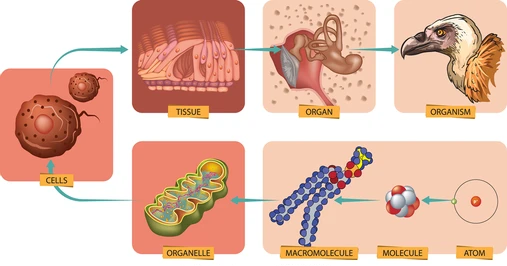
\includegraphics{res/proteins_overview/atom_bird.png}
    \caption{Atom to macromolecules to organism}
    \label{fig:atom-bird}
\end{figure}

In figure \ref{fig:atom-bird} we can see the various steps from molecules to macromolecules to bigger complexes up to the final organism.

The passage between molecules to macromolecules, can be observed more in detail in the following figure.
\begin{figure}[h!]
    \centering
    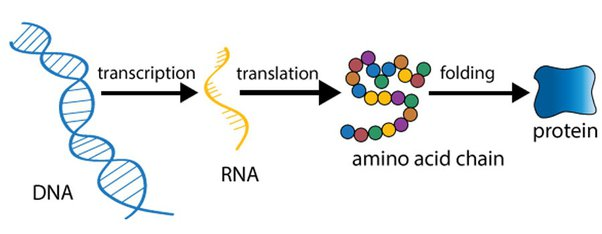
\includegraphics{res/proteins_overview/dna_protein.png}
    \caption{Atom to macromolecules to organism}
    \label{fig:molecule-protein}
\end{figure}

In figure \ref{fig:molecule-protein} we can see the passages and we can observe each structure from DNA to RNA to peptide chains to protein. We already explained earlier the phases of transcription, translation and folding in chapter \ref{sec:central-dogma}. 

We can use structural data for:
\begin{itemize}
    \item Structure prediction;
    \item Predicting protein interactions: protein folding, binding, protein assemblies;
    \item Structure comparison: by comparing the moolecules' structure we can determine to which species it belongs to and where in the evolutionary scale it stands;
    \item Exploring mechanisms of interaction with ligands: metabolites, drug compounds, DNA and others.
\end{itemize}

From molecular data we get information on coordinates and then we want to obtain some kind of knowledge, for example:
\begin{itemize}
    \item Mutation X disrupts the function of enzyme Y which causes disease Z.
\end{itemize}

\vspace{1em}

\noindent "Coordinates by themselves just specify shape and are not necessarily of intrinsic biological value, unless they can be related to other information"

\noindent \small{\textit{Integrative database analysis in structural genomics, Mark Gerstein, Nature Structural Biology}}

\normalsize{There are many databases that store information on structural data for many proteins or other macromolecules, some of them also contains sequence data or metabolic pathways data. Sequence data are just data on DNA so the sequences, while metabolic pathways are related to which pathway a given gene activate.}

Down below we can see a picture of most databases for bioinformatics data.
\begin{figure}[h!]
    \centering
    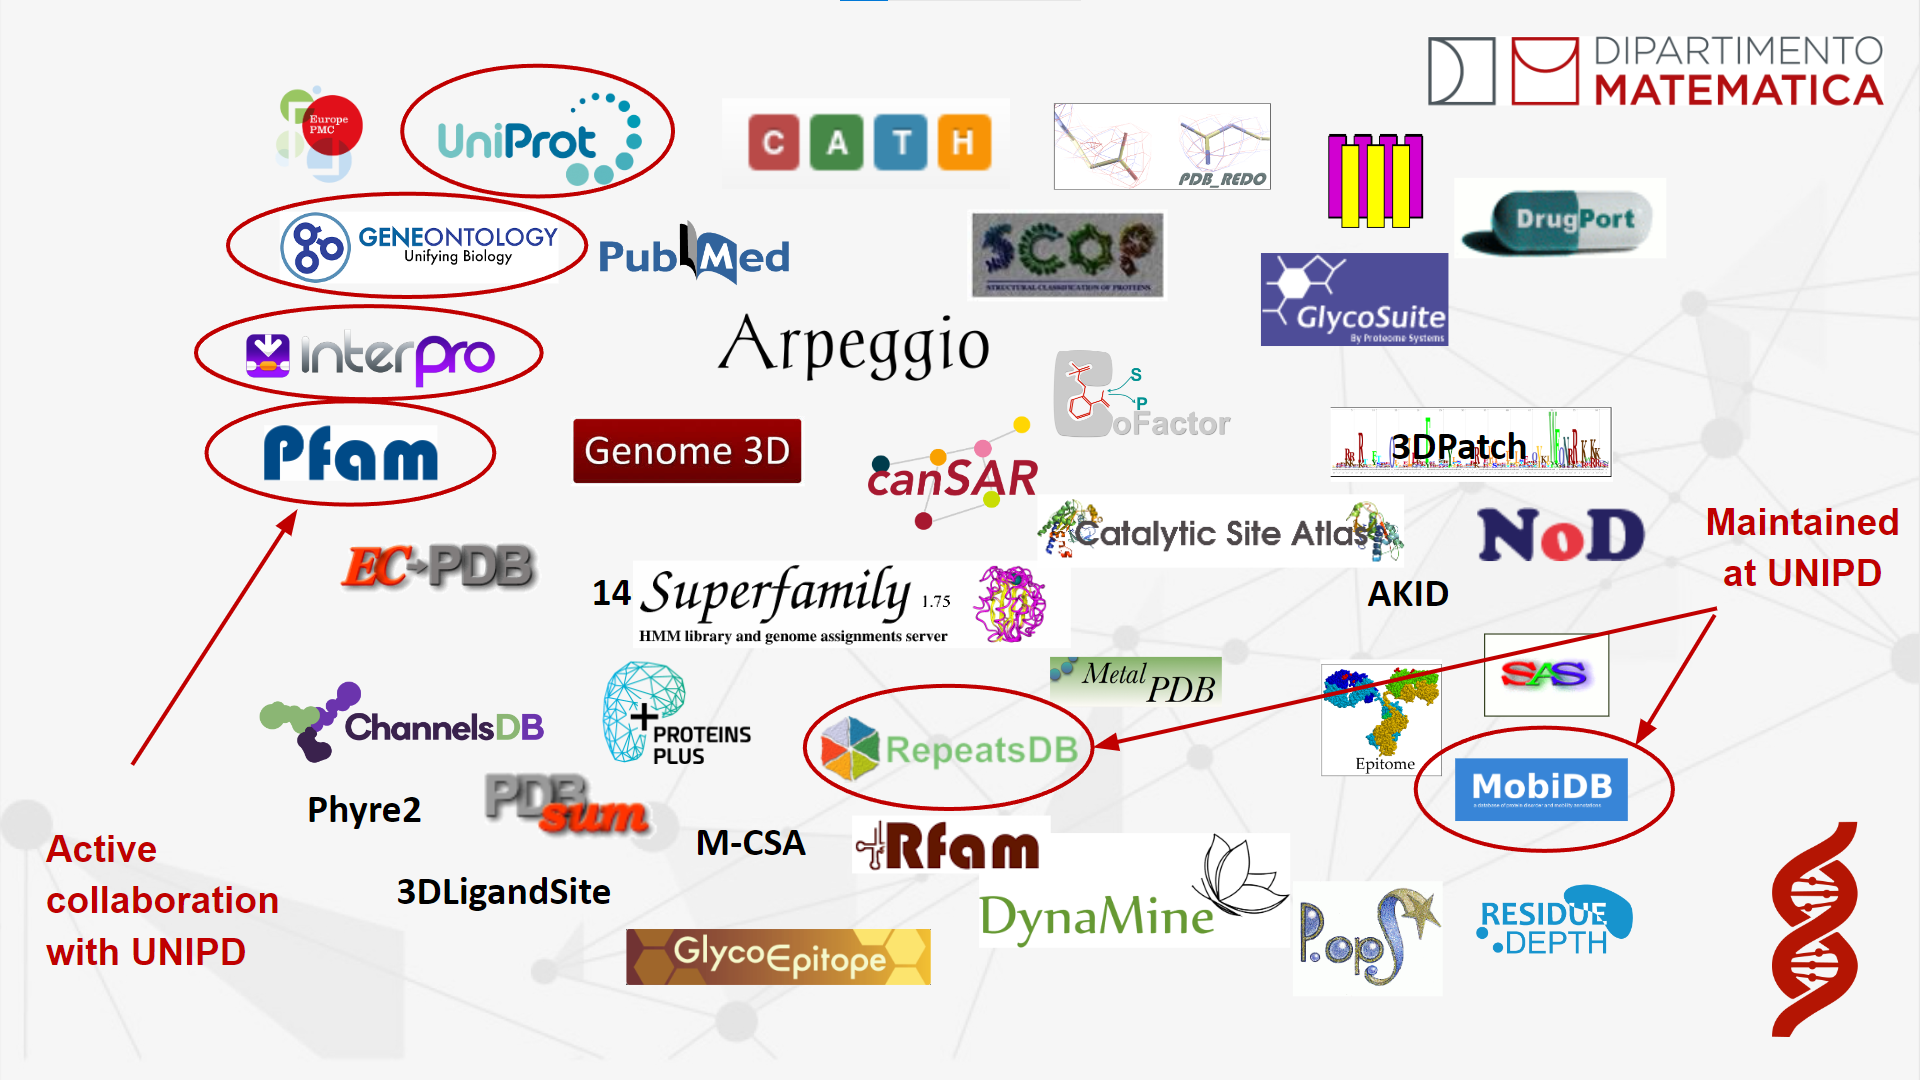
\includegraphics[scale=0.3]{res/proteins_overview/pdb.png}
    \caption{PDB-derived databases}
\end{figure}

These are all PDB-derived databases, since PDB (Protein Data Bank) was one of the first to try and build up an archive on protein structural data, and so all these databases are derived from the PDB archive.

Lastly, we can see a figure representing the most used biological technologies for obtaining structural data.

\begin{figure}[h!]
    \centering
    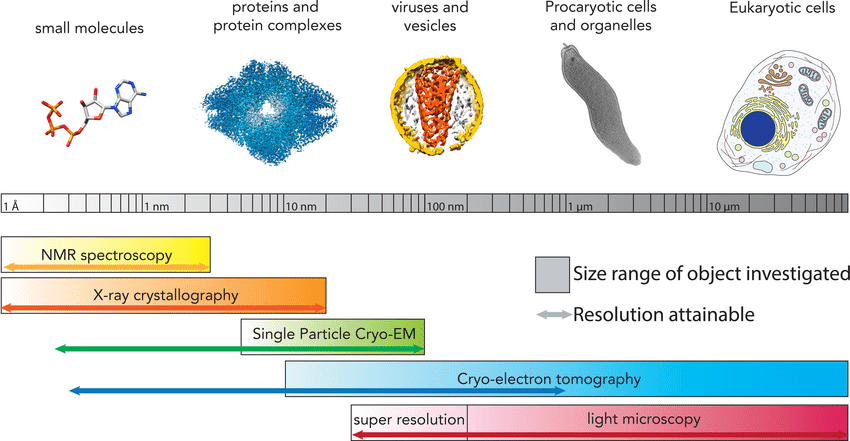
\includegraphics[scale=0.6]{res/proteins_overview/methods_structural.png}
    \caption{Biological technologies for obtaining structural data}
\end{figure}

In our case, for protein chains and residues, the most interesting biological technologies are the first two from left:
\begin{itemize}
    \item X-ray crystallography;
    \item NMR spectroscopy.
\end{itemize}

To close up this chapter I will talk about one of the most important libraries in bioinformatics: BioPython.
\subsection{BioPython}
Regarding Computer Science the main languages used for bioinformatics are:
\begin{itemize}
    \item R;
    \item Matlab;
    \item Python.
\end{itemize}
For python there is the library BioPython, which is a library containing classes, functions and modules for the various necessities in bioinformatics.

\begin{figure}[h!]
    \centering
    
\includegraphics{res/proteins_overview/biopython.png}
\end{figure}

There are a lot of subpackages under the package Bio of BioPython, in our case we are just interested in 3 of them:
\begin{itemize}
    \item \textbf{Bio.PDB}: contains classes that deal with macromolecular crystal structures. In particular it includes PDB and mmCIF parsers, the DSSP wrapper\footnote{A wrapper is a class or procedure that translates a library's existing interface into a compatible interface, it "wraps" the underlying library. It's often used to enable cross-language, in this case the wrapper enables the c++ library "DSSP" to be used in Python.}, the SASA module and the Structure class;
    \item \textbf{Bio.Data}: collection of useful biological data, for example in our case we use it for the normalization factors for RSA;
    \item \textbf{Bio.SeqUtils}: contains mhelper functions to deal with sequences.
\end{itemize}

In particular from Bio.PDB we use the classes:
\begin{itemize}
    \item \textit{PDBParser}: as the name suggests, it's a class which reads a .pdb file and saves it into a variable of the type Structure class;
    \item \textit{MMCIFParser}: similar to PDBParser, but for .mmCIF files;
    \item \textit{DSSP}: the python wrapper for the software tool DSSP;
    \item \textit{SASA}: a class for calculating solvent accessibility;
    \item \textit{Polypeptide}: a class with helper functions to deal with protein chains, in particular we use the function \textbf{is\_aa()} to see if a string is an identifier for an amino acid.
\end{itemize}

On the other hand the Bio.Data subpackage has been used just for the normalization factors for SASA, the dictionary \textit{residue\_sasa\_scales}. 

And Bio.SeqUtils has been used for the helper function \textit{Seq1}, which converts a sequence of amino acids with three-letters code into a sequence of amino acids with one-letter code.

For more information on BioPython and its subpackages and submodules, here is the link to the  \underline{\href{https://biopython.org/docs/dev/api/index.html}{documentation}}.